Let $y$ be the position of a particle in one dimension, and let $t$ be time. So
there is just a single input variable: $t$.

An Ordinary Differential Equation is an equation relating the input variable
$t$ to $y$ and its derivatives. So, in general,
\begin{align*}
  f\(t, y, y', y'', \ldots\) = 0.
\end{align*}

A first-order ODE involves first derivatives only.

Consider the subset\footnote{I.e. $f(t, y, y') = 0$ can be rearranged to give
  $y'$ as a function of $t, y$.} of first-order ODEs that specify a velocity
$v(t, y)$ at each point in $(t, y)$ space. Thus this ODE contains all the
information needed to animate the motion of the particle, starting from any
point $(t_0, y_0)$. So the statement of the initial condition problem is
\begin{align*}
  \dydt = v(t, y) ~~~~~~~~~~ y(t_0) = y_0.
\end{align*}

The solution to an ODE is a function $y = \varphi(t)$ that describes a motion
of the particle having the specified velocities at each point it passes
through. I.e., if $y = \varphi(t)$ is a solution, then
\begin{align*}
  \frac{\d \varphi}{\dt} = v\Big(t, \varphi(t)\Big) ~~~~~~~~~~~~~\text{for all $t$}.
\end{align*}

The phase space of this problem is the set of all possible $(y, v)$ values.?

\section{Special cases}
\subsection{Velocity depends on time only}
\begin{align*}
  \dydt = v(t)
\end{align*}
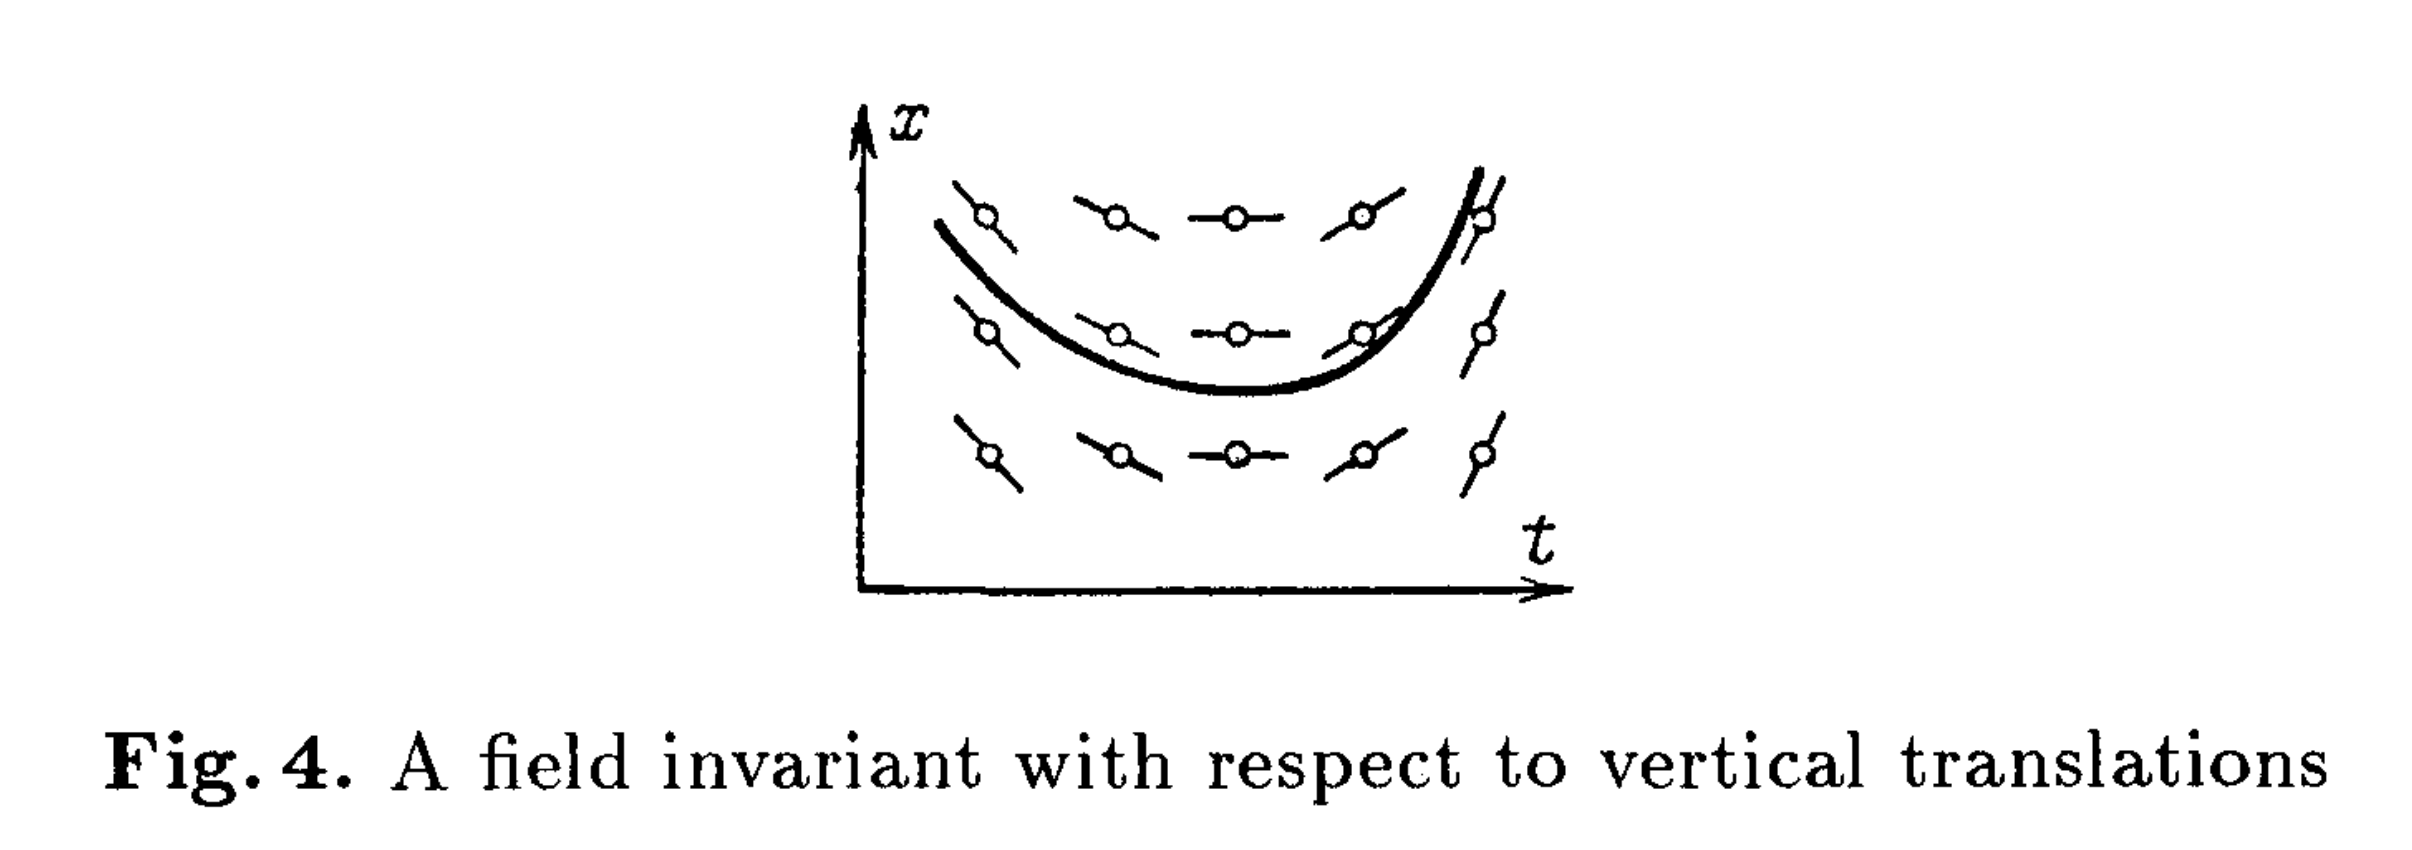
\includegraphics[width=340pt]{img/differential-equations-1-direction-field.png}\\
To find functions that solves this, one possibility is that we can find the
antiderivative explicitly:
\begin{align*}
  \int \dydt \dt := y(t) + C = \int v(t) \dt.
\end{align*}


\subsection{Velocity depends on location only (autonomous)}
\begin{align*}
  \dydt = v(y)
\end{align*}
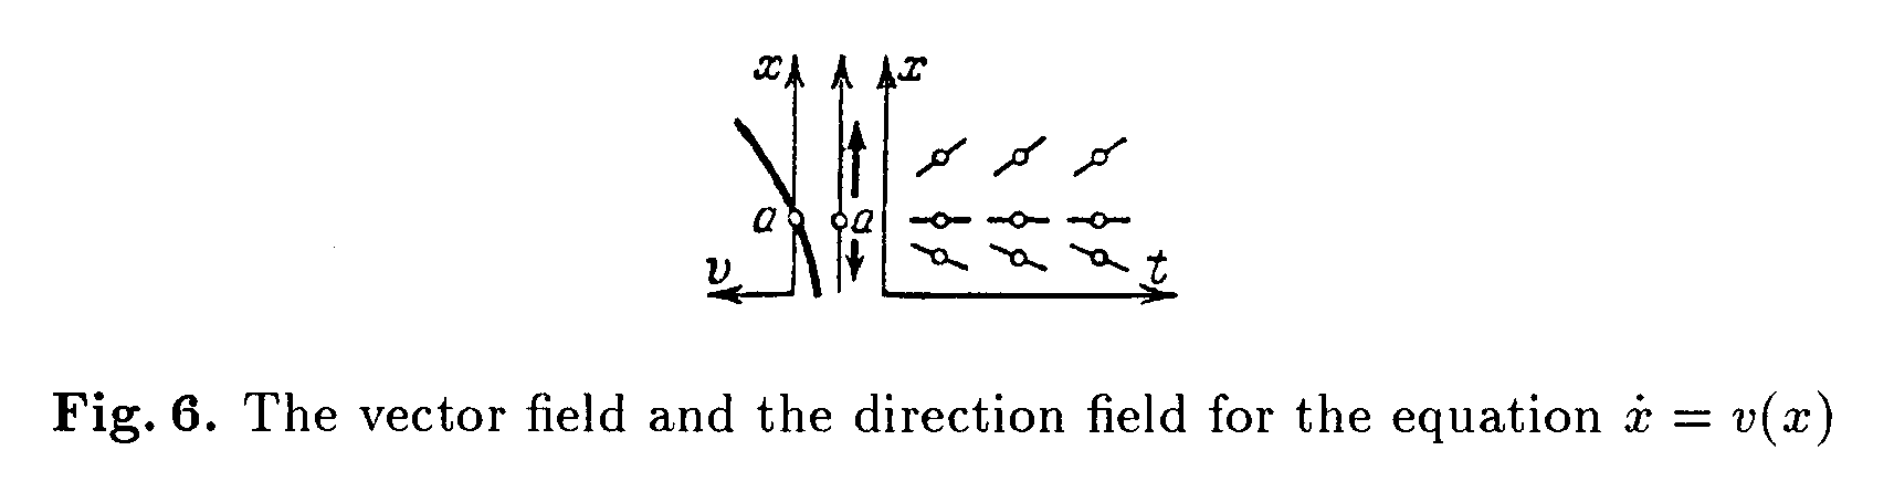
\includegraphics[width=400pt]{img/differential-equations-2-direction-field.png}\\



\section{Examples}
\subsection{C$^{14}$ dating}
\begin{mdframed}
  In a living organism the amount of C$^{14}$, as a proportion of all the
  C$^{12}$ and C$^{14}$, is expected to be a known constant $p_0$. After death,
  C$^{14}$ decays to C$^{12}$. How old is a specimen with proportion $p_1$ of
  C$^{14}$?
\end{mdframed}
Let $\lambda$ be the rate at which one atom of C$^{14}$ decays in atoms/sec. So
in a sample of $N$ atoms, the expected number to decay in one second is
$N\lambda$.

Let $N(t)$ be the number of C$^{14}$ atoms remaining at time $t$. We can
specify the model as a first-order ODE:
\begin{align*}
\frac{\d N}{\dt} = -N\lambda.
\end{align*}
Equivalently, dividing by the constant total number of carbon atoms,
\begin{align*}
\frac{\d p}{\dt} = -p\lambda,
\end{align*}
where $p(t)$ is the proportion of C$^{14}$ at time $t$.

It's easy to find a family of functions $p(t)$ that satisfies this differential equation. Since
\begin{align*}
  \frac{1}{p(t)} \frac{\d p}{\dt} = -\lambda,
\end{align*}
it must be the case that their antiderivatives are the same, up to a constant:
\begin{align*}
  \log(p(t)) &= -\lambda t + C\\
  p(t)  &= Ae^{-\lambda t}.
\end{align*}
Further, the expected proportion in a living organism determines a particular
function as the solution:
\begin{align*}
  p(0) = p_0 = Ae^{-\lambda . 0}
\end{align*}
so $A = p_0$ and the solution is
\begin{align*}
  p(t)  &= p_0e^{-\lambda t}.
\end{align*}
So the estimated age of a sample with proportion $p_1$ is
\begin{align*}
  t = \frac{1}{\lambda}\log\(\frac{p_0}{p_1}\).
\end{align*}



\section{Picard's Existence Theorem}
Consider again the initial condition problem
\begin{align*}
  \dydt = v(t, y) ~~~~~~~~~~ y(t_0) = y_0.
\end{align*}


The ODE could also be written as
\begin{align*}
  y(t) = \int v\Big(t, y(t)\Big) \dt + C,
\end{align*}
but this is merely an equivalent restatement, since the definition of
indefinite integral is antiderivative. If we can find an antiderivative, then
fine. If not, note that by FTC, the following definite integral describes a
solution:
\begin{align*}
  y(t) = y(t_0) + \int_{t_0}^t v\Big(\tau, y(\tau)\Big) \d\tau.
\end{align*}
But this specifies $y(t)$ in terms of itself, since the velocity $v$ depends
not only on $t$ but also on the current position\footnote{for example, the rate
  of change of the proportion on carbon-14 depends on the current proportion of
  carbon-14.}.

\theorem{The following sequence of functions converges to a unique solution:
  \begin{align*}
    y_0(t) &= y(t_0)\\
    y_n(t) &= y(t_0) + \int_{t_0}^t v\Big(\tau, y_{n-1}(\tau)\Big) \d\tau.\\
  \end{align*}
}

\proof{}
We show
\begin{enumerate}
\item The $y_n(t)$ converge to a function $y(t)$
\item This function is a solution
\item It is unique
\end{enumerate}

\subsection{Proof that the $y_n(t)$ converge to a function $y(t)$}

Note that the

Define $e_n(t) = y_n(t) - y_{n-1}(t)$ and note that $y_n(t) = y(t_0) + \sum_{i=1}^n e_n(t)$.
\begin{align*}

\end{align*}

\newpage
\section{Simmons}

\subsection{Picard's theorem}
For every point $(t, y)$ in a rectangle, the ODE
\begin{align*}
  \dydt = f(t, y)
\end{align*}
has a solution passing through that point if $\partiald{f}{y}$ is Lipschitz
continuous in that rectangle.

\subsection{Families of curves}
For a family of curves, say the family of circles
\begin{align}
  x^2 + y^2 = c^2 \label{simmons-circles}
\end{align}
we can obtain a differential equation by implicit differentiation:
\begin{align}
  2x + 2y\dydx = 0. \label{simmons-circles-de}
\end{align}
Alternatively (eoc),
\begin{align*}
  (x + \dx)^2 + (y + \dy)^2 &= c^2\\
  x^2 + 2x\dx + y^2 + 2y\dy &= c^2\\
        2x\dx  + 2y\dy     &= 0.
\end{align*}

\subsection{Orthogonal trajectories}
What's the family of curves each of which is equal to every circle in \eqref{simmons-circles}?

Well, we know that their gradients are negative the inverse of the circle
gradients. So if we let $\dydx$ now be the gradient of the orthogonal
trajectories, then from \eqref{simmons-circles-de},
\begin{align*}
  2x - 2y\dxdy = 0
\end{align*}
is an ODE specifying the family of orthogonal trajectories. Thus
\begin{align*}
  \dydx &= \frac{y}{x}\\
  \log(y) &= \log(x) + C\\
       y &= Ax,
\end{align*}
so the orthogonal trajectories are lines through the origin, as expected.

\subsection{Use of polar coordinates to make a problem tractable (separable)}
TODO

% \section{Arnold - Problems}
% \subsection{}
% \begin{mdframed}
%   At what altitude is the density of the air one half of that at the surface of
%   the Earth? Regard temperature as constant. One cubic meter of air at the
%   Earth's surface weighs 1250g.
% \end{mdframed}
% \begin{align*}
%   \rho(0) = 1250\\
%   &=
% \end{align*}